% This must be in the first 5 lines to tell arXiv to use pdfLaTeX, which is strongly recommended.
\pdfoutput=1
% In particular, the hyperref package requires pdfLaTeX in order to break URLs across lines.

\documentclass[11pt]{article}

% Change "review" to "final" to generate the final (sometimes called camera-ready) version.
% Change to "preprint" to generate a non-anonymous version with page numbers.
\usepackage[final]{acl}

% Standard package includes
\usepackage{times}
\usepackage{latexsym}

% For proper rendering and hyphenation of words containing Latin characters (including in bib files)
\usepackage[T1]{fontenc}
% For Vietnamese characters
% \usepackage[T5]{fontenc}
% See https://www.latex-project.org/help/documentation/encguide.pdf for other character sets

% This assumes your files are encoded as UTF8
\usepackage[utf8]{inputenc}

% This is not strictly necessary, and may be commented out,
% but it will improve the layout of the manuscript,
% and will typically save some space.
\usepackage{microtype}

% This is also not strictly necessary, and may be commented out.
% However, it will improve the aesthetics of text in
% the typewriter font.
\usepackage{inconsolata}

% If the title and author information does not fit in the area allocated, uncomment the following
%
%\setlength\titlebox{<dim>}
%
% and set <dim> to something 5cm or larger.
\usepackage{diagbox}

\usepackage{tikz}
\usetikzlibrary{shapes.geometric, arrows, positioning}
\usepackage{tikzscale}
\usepackage{longtable}
\usepackage{graphicx}
\usepackage{tabularx}
\usepackage{array}
\usepackage{subcaption}
\usepackage{pgfplots}
\usepackage{afterpage}
\usepgfplotslibrary{groupplots}
\usepgfplotslibrary{colorbrewer}
% \usepackage{tikz}
\usepackage{booktabs}
\usepackage{multirow}
\usepackage{xcolor}
% \usetikzlibrary{matrix}
% \usepackage{hyperref}


%\title{Artificial Authorship: Refining Detection and Explanation in Machine-Generated Texts}
\title{``I know myself better, but not really greatly'': Using LLMs to Detect and Explain LLM-Generated Texts}

% Author information can be set in various styles:
% For several authors from the same institution:
% \author{Author 1 \and ... \and Author n \\
%         Address line \\ ... \\ Address line}
% if the names do not fit well on one line use
%         Author 1 \\ {\bf Author 2} \\ ... \\ {\bf Author n} \\
% For authors from different institutions:
% \author{Author 1 \\ Address line \\  ... \\ Address line
%         \And  ... \And
%         Author n \\ Address line \\ ... \\ Address line}
% To start a separate ``row'' of authors use \AND, as in
% \author{Author 1 \\ Address line \\  ... \\ Address line
%         \AND
%         Author 2 \\ Address line \\ ... \\ Address line \And
%         Author 3 \\ Address line \\ ... \\ Address line}

\author{Jiazhou Ji$^{1\ast}$ \quad Jie Guo$^{1}\thanks{Equal contributions.}$ \quad Weidong Qiu$^{1}$\quad Zheng Huang$^{1}$ \quad Yang Xu$^{1}$ \\\textbf{Xinru Lu$^{1}$ \quad Xiaoyu Jiang$^{1}$ \quad Ruizhe Li$^{2\dag}$\quad Shujun Li$^{3}\thanks{Corresponding co-authors: \texttt{ruizhe.li@abdn.ac.uk, s.j.li@kent.ac.uk}}$} \\
$^1$School of Cyber Science and Engineering, Shanghai Jiao Tong University, China\\ $^2$Department of Computing Science, University of Aberdeen, UK\\ $^3$Institute of Cyber Security for Society (iCSS) \& School of Computing, University of Kent, UK\\
}

\begin{document}

\maketitle

\begin{abstract}
Large language models (LLMs) have demonstrated impressive capabilities in generating human-like texts, but the potential misuse of such LLM-generated texts raises the need to distinguish between human-generated and LLM-generated content. This paper explores the detection and explanation capabilities of LLM-based detectors of LLM-generated texts, in the context of a binary classification task (human-generated texts vs LLM-generated texts) and a ternary classification task (human-generated texts, LLM-generated texts, and undecided). By evaluating on six close/open-source LLMs with different sizes, our findings reveal that while self-detection consistently outperforms cross-detection, i.e., LLMs can detect texts generated by themselves more accurately than those generated by other LLMs, the performance of self-detection is still far from ideal, indicating that further improvements are needed. We also show that extending the binary to the ternary classification task with a new class ``Undecided'' can enhance both detection accuracy and explanation quality, with improvements being statistically significant and consistent across all LLMs. We finally conducted comprehensive qualitative and quantitative analyses on the explanation errors, which are categorized into three types: reliance on inaccurate features (the most frequent error), hallucinations, and incorrect reasoning. These findings with our human-annotated dataset emphasize the need for further research into improving both self-detection and self-explanation, particularly to address overfitting issues that may hinder generalization.
% \noindent\textbf{Key words: }machine-generated text detection, ternary classification, explainability
\end{abstract}

\section{Introduction}

The rise of large language models (LLMs) has brought remarkable advancements in natural language processing (NLP) tasks \cite{matarazzo2025survey}, including text generation. Models such as GPT-4o \cite{OpenAI2024GTP4O}, LLaMA \cite{Touvron2023LLaMA}, and Qwen \cite{ali2024qwen2} have blurred the boundaries between LLM-generated (LGTs) and human-generated texts (HGTs), posing new challenges in distinguishing between the two. While these capabilities of LLMs open new possibilities, they also bring concerns in areas such as misinformation, academic dishonesty, and automated content moderation \cite{hu2025unveiling}. As a result, detecting LGTs has become an increasingly important research area \cite{dugan2024raid, lee2023do, bhattacharjee2024fighting}.

Prior research has primarily focused on developing classifiers to distinguish HGTs and LGTs, including open-source detectors~\cite{Hans2024Binoculars} and online close-source detection systems~\cite{gptzero_website}. However, most detection systems have been limited to binary classification, which has several inherent issues. Recently, some works~\cite{lee2024llm} have attempted ternary classification by introducing a ``mixed'' category, which represents texts originating from mixed sources. However, this approach does not fundamentally resolve the issue. We further adopt the definition of an ``Undecided'' category based on other studies~\cite{ji2024detecting} and conduct ternary classification experiments for different LLMs, as certain texts are inherently indistinguishable between LGTs and HGTs. Furthermore, many studies treat the detection task as a black box, offering little insight into the decision-making process. Explainability, a critical aspect of trustworthy AI, has received less attention, but it is essential for building systems that users can trust \cite{weng2024understanding, zhou2024humanizing}. This paper presents an analysis of LLMs in detecting LGTs and HGTs, with a particular emphasis on evaluating and improving the clarity of the explanations provided by LLM-based detectors. By investigating how LLMs make predictions and offer explanations for their decisions, we aim to enhance their transparency and provide deeper insights into their reasoning processes.

This paper explores the explainability of LLM-based detectors, addressing two central questions: (1) How accurately can detectors identify the origins of texts, and (2) How reliable are their explanations? Our study highlights that in a ternary setting compared to traditional binary classification, the average detection performance improves by 5.6\%, which demonstrates the necessity of ternary rather than binary setting to detect HGTs and LGTs. We further discovered that explanations are often flawed even when binary predictions are correct. Based on our comprehensive human-annotators' feedback, we summarize three common issues with explanations: reliance on inaccurate features (e.g., vague or irrelevant characteristics), hallucinations (e.g., non-existent or contradictory features), and incorrect reasoning (e.g., logical errors in attributing text origin). These explanation errors are quantified and categorized, with their distributions analyzed across different LLMs. Consequently, the proportion of explanation errors decreases by 13.3\% when we switch to the ternary classification setting, which further supports the necessity of ternary classification for LGTs detection.

In our experiments, we evaluated six state-of-the-art (SOTA) LLM-based detectors, such as GPT-4o, GPT-4o mini, LLaMA3.3-70B, LLaMA3.3-7B, Qwen2-72B, and Qwen2-7B, on our created benchmark dataset comprising LGTs and HGTs. Moreover, our human annotators provided feedback based on the correctness of predictions and explanations for this benchmark. Our results show that GPT-4o achieved the highest detection accuracy. In addition, LLMs performed better in self-detection than cross-detection, and ternary classification outperformed binary classification. Finally, explanation quality also improved under the ternary setting, with fewer hallucinations and incorrect reasoning observed.

The contributions of this paper are threefold:
\begin{itemize}
\item \textbf{Evaluation of Binary and Ternary Classification for Detection and Explanation:} We evaluate LLM-based detectors with both binary and ternary classification tasks, showing that self-detection outperforms cross-detection, and detection accuracy is higher within the same model family. We also demonstrate that ternary classification improves both detection and explanation quality, providing a more nuanced understanding of text origins.

\item \textbf{Human-Annotated Dataset for Explanation Evaluation and Detector Training:} We introduce a human-annotated dataset of LGTs and HGTs for evaluating LLM explanations and training detectors. This resource improves model performance by offering insights into reasoning processes\footnote{Our human-annotated dataset regarding LLM-based self-detection and cross-detection with explanations will be public available after acceptance.}.

\item \textbf{Quantitative and Qualitative Analysis of Explanation Errors:} We identify three main explanation errors, i.e., reliance on inaccurate features, hallucinations, and incorrect reasoning, and quantify their occurrence across models and tasks. This analysis provides insights for improving LLM detection and reasoning capabilities.
\end{itemize}

\section{Related Work}

\paragraph{LGT and HGT Detection.}
Past efforts to identify LLM-generated texts (LGTs) often relied on binary classification systems that distinguish human-generated texts (HGTs) from LGTs using surface-level features. While these methods were initially effective, they are prone to errors when encountering adversarial attacks or domain shifts, which limit their overall robustness~\cite{bhattacharjee2024fighting, dugan2024raid}. To address these limitations, researchers have explored strategies that integrate external knowledge, such as combining internal and external factual structures, to boost detection against diverse content and styles~\cite{ideate2024}. Recent studies also highlight the promise of using the LLMs themselves for text detection: approaches like self-detection and mutual detection can outperform traditional classifiers, as illustrated by GPT-4's success in tasks like plagiarism detection~\cite{plagbench2024}. Notably, smaller models sometimes excel in zero-shot scenarios, offering adaptable solutions across varying architectures~\cite{smallerLLM2024}. Furthermore, \citet{lee2023do} demonstrated that LLMs can reliably identify their own outputs, providing a more nuanced framework for content verification. Despite these advances, the continuing challenges of domain adaptation and adversarial resistance underscore the need for more versatile and robust detection systems.



\textbf{Explainability in Detection Models.}
Recent work on LGT detection has focused on improving explainability. \citet{zhou2024humanizing} proposed to incorporate factual consistency into detection models to enhance their interpretability, while~\citet{weng2024understanding} explored mixed-initiative approaches that combine human expertise with automated models for better detection. These studies have made significant contributions to the field; however, they either depend heavily on expert input~\cite{weng2024understanding} or lack integration of explanation generation within the model itself~\cite{zhou2024humanizing}. Our approach, in contrast, enables LLMs to autonomously generate both predictions and detailed explanations, making it a more scalable and transparent solution for detecting machine-generated content.

\textbf{Ternary Classification.}
Traditional binary classification methods, distinguishing between LGTs and HGTs, face limitations when texts exhibit characteristics that are ambiguous or could plausibly originate from either source. In such cases, adding an ``Undecided'' category provides a more nuanced framework for detection. This approach has several advantages over previous methods, which typically focus on mixed human-machine texts and fail to account for uncertainties in text origin. For instance, the work by~\citet{lee2024llm} revealed that current detectors struggle to identify ``mixed text'', particularly in cases where subtle modifications and style adaptability blur the distinction. Similarly, the Turing test conducted on online reviews~\cite{turingtest2024} showed that even humans often cannot reliably distinguish between human-written and AI-generated content, pointing to the inherent difficulties in binary classification. Moreover, studies such as~\cite{turingtest2024} and \cite{coling2024} further underscore the complexity in distinguishing between the two, suggesting that an ``Undecided'' class could allow for better handling of such ambiguity. Incorporating this third category not only enhances detection accuracy but also improves explainability, offering clearer insights into the decision-making process.

\section{LLM-based Binary Classification on LGTs and HGTs}
\label{sec:binary_classification}



\subsection{Experimental Design}

We selected six SOTA LLMs for text generation and subsequent detection: GPT-4o, GPT-4o mini~\cite{hurst2024gpt}, Qwen2-72B, Qwen2-7B~\cite{yang2024qwen2}, LLaMA3.3-70B, and LLaMA3.3-8B~\cite{dubey2024llama}. These LLMs were chosen for two main reasons. First, they represent the latest advancements in LLM development, demonstrating strong generation and detection capabilities. Second, the selection spans different series and model sizes, enabling a comparative analysis of performance across architectures and scales.

To construct the dataset, we first selected 1,000 HGTs from the publicly available M4GT-Bench dataset~\cite{wang2024m4gt}, ensuring a diverse range of topics, styles, and formats. Based on these selected HGTs, we then designed 1,000 prompts that align with the themes, structure, and style of the HGTs. Each LLM subsequently generated a corresponding response for each of these prompts. Together, these LGTs and HGTs formed the benchmark used in this study. For each text, the LLMs were tasked to determine its source (LGTs or HGTs) and provide an explanation, as illustrated in Table~\ref{tab:prompt_binary_classification}.

\begin{table}[h]
\centering
\small
\begin{tabular}{@{}p{\linewidth}@{}} % 使用p{width}指定每列宽度
\toprule
\textbf{Prompt}: Please determine whether the following text is generated by large language models or by a human, and provide a clear judgment. Additionally, please offer a detailed explanation for your decision. Please structure your answer in JSON format as follows: \{``answer'': , ``explanation'': \}.\\
\bottomrule
\end{tabular}
\caption{A prompt designed for LLMs to determine the origin of a text and provide an explanation under a binary setting.}
% \vspace{-2em}
\label{tab:prompt_binary_classification}
\end{table}

\paragraph{Manual Annotation.} To assess LLMs' ability to explain text origins and identify distinguishing features, three co-authors, who are undergraduate Computer Science students, manually evaluated the correctness of LLM-generated explanations. They determined whether each explanation was accurate or inaccurate. From seven datasets (6 SOTA LLMs + Human), 100 texts with the corresponding explanations per dataset were randomly selected for human evaluation. All annotators assessed the explanations provided by each model, which achieved a Fleiss' kappa~\cite{Fleiss1971kappa} of 0.8387, indicating near-complete agreement. Annotation guidelines are detailed in Appendix~\ref{appendix:annotation_guidelines}.

\begin{table*}[tb]
\centering
\small
% \setlength{\tabcolsep}{3pt}
% \begin{tabularx}{\textwidth}{@{}c *{6}{>{\centering\arraybackslash}X} @{}}
\resizebox{\textwidth}{!}{
\begin{tabular}{lcccccc}
\toprule
\multirow{2}{*}{\diagbox{Datasets}{Models}} & \multicolumn{6}{c}{LLM Detectors}\\
& GPT-4o & GPT-4o mini & LLaMA3.3-70B & LLaMA3.3-8B & Qwen2-72B & Qwen2-7B \\
\midrule
\textbf{GPT-4o}      & 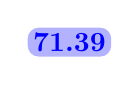
\begin{tikzpicture}[baseline=(X.base)]
\node[fill=blue!30, inner sep=2pt, rounded corners] (X) {\textcolor{blue}{\textbf{71.39}}};\end{tikzpicture} & 59.38 & 57.31 & 48.41 & 64.14 & 59.76 \\ 
\textbf{GPT-4o mini}   & 65.71 & 61.03 & 53.75 & 51.73 & \textcolor{blue}{\textbf{67.27}} & 60.09 \\ 
\textbf{LLaMA3.3-70B}   & \textcolor{blue}{\textbf{67.26}} & 60.92 & 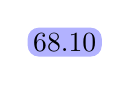
\begin{tikzpicture}[baseline=(X.base)]
\node[fill=blue!30, inner sep=2pt, rounded corners] (X) {68.10};\end{tikzpicture} & 53.65 & 58.96 & 51.57 \\ 
\textbf{LLaMA3.3-8B}    & 60.74 & 55.77 & \textcolor{blue}{\textbf{62.29}} & 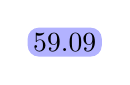
\begin{tikzpicture}[baseline=(X.base)]
\node[fill=blue!30, inner sep=2pt, rounded corners] (X) {59.09};\end{tikzpicture} & 59.87 & 49.88 \\ 
\textbf{Qwen2-72B}      & 62.66 & 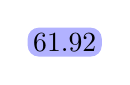
\begin{tikzpicture}[baseline=(X.base)]
\node[fill=blue!30, inner sep=2pt, rounded corners] (X) {61.92};\end{tikzpicture} & 57.79 & 49.20 & 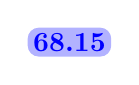
\begin{tikzpicture}[baseline=(X.base)]
\node[fill=blue!30, inner sep=2pt, rounded corners] (X) {\textcolor{blue}{\textbf{68.15}}};\end{tikzpicture} & 61.36 \\ 
\textbf{Qwen2-7B}       & 62.45 & 59.06 & 59.12 & 48.57 & \textcolor{blue}{\textbf{65.24}} & 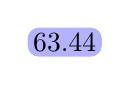
\begin{tikzpicture}[baseline=(X.base)]
\node[fill=blue!30, inner sep=2pt, rounded corners] (X) {63.44};\end{tikzpicture} \\\midrule 
\textbf{Average}        & \textcolor{blue}{\textbf{65.03}} & 59.68 & 59.73 & 51.78 & 63.94 & 57.68 \\ 
\bottomrule
\end{tabular}}
\caption{F1 scores of LLM-based detectors in binary classification. The first column indicates different LLMs used for text generation, and the first row indicates different LLMs acting as detectors. The highest column-wise F1 score for each LLM detector to classify LGTs and HGTs across six datasets is highlighted in \colorbox{blue!30}{blue}. The highest row-wise F1 score for each LLM-generated text dataset across different LLM detectors is marked in \textcolor{blue}{\textbf{blue}}.}
% \vspace{-1.5em}
\label{tab:binary_gt_performance}
\end{table*}

\paragraph{Evaluation Metrics.} For evaluating the classification performance of the LLMs, the primary metric we used is the F1 score. To assess the quality of explanations, human evaluators reviewed the LLM-generated explanations and classified them as correct or incorrect. The F1 score was also used as the evaluation metric for explanation quality.

\subsection{Binary Classification Results}

We evaluated the performance of six LLMs across six datasets, as detailed in Table~\ref{tab:binary_gt_performance}, which systematically compares the detection capabilities of various LLMs for both LGTs and HGTs. The results demonstrate that GPT-4o achieves the best average detection performance across all datasets, showing relatively strong generalization capabilities. Larger parameter models generally exhibit significantly better detection performance than smaller ones, which suggests that these models are not merely making random guesses but are effectively identifying distinctive textual features.

The \colorbox{blue!30}{F1 scores} in Table~\ref{tab:binary_gt_performance}'s diagonal direction show that LLMs within the same series consistently detect their own outputs more effectively than those from other LLM families. For example, LLaMA3.3 70B achieves the highest \colorbox{blue!30}{F1 score} in its generated dataset, which indicates a heightened sensitivity to its own text distribution compared to other LLMs. However, this specialization reduces cross-detection performance, as seen in Qwen2-7B's lower F1 on LLaMA-generated texts. While larger LLMs generally achieve better detection across different LLMs, such as GPT-4o, GPT-4o mini, LLaMA3.3-70B and Qwen2-72B, their outputs are also more difficulty to distinguish by smaller LLMs, such as LLaMA3.3-8B and Qwen2-7B.

Additionally, based on the human annotations of sampled 100 LGTs and 100 HGTs with explanations from each dataset, we observed that the detection and explanation results across different LLMs are not entirely consistent, as shown in Table~\ref{tab:binary_annotate_performance}. We noted that in some cases, the F1 score for explanations was higher than that for classification. This is because, in these cases, the explanation correctly identified the reasoning for attribution, but the final classification was incorrect. For instance, the difference in F1 scores between explanation and classification was particularly noticeable for LLaMA3.3-8B and Qwen2-7B, suggesting that these models struggle to truly comprehend the textual features necessary for correctly determining the origin of generated texts, which results in lower detection performance.

\begin{table*}[tb]
\centering
\small
% \setlength{\tabcolsep}{3pt}
% \begin{tabularx}{\textwidth}{@{}c *{6}{>{\centering\arraybackslash}X} @{}}
\resizebox{\textwidth}{!}{
\begin{tabular}{lcccccc}
\toprule
\multirow{2}{*}{\diagbox{Datasets}{Models}} & \multicolumn{6}{c}{LLM Detectors}\\
& GPT-4o & GPT-4o mini & LLaMA3.3-70B & LLaMA3.3-8B & Qwen2-72B & Qwen2-7B \\
\midrule
\textbf{GPT-4o}      & 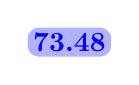
\begin{tikzpicture}[baseline=(X.base)]
\node[fill=blue!30, inner sep=2pt, rounded corners] (X) {\textcolor{blue}{\textbf{73.48}}};\end{tikzpicture}
/ 
\begin{tikzpicture}[baseline=(X.base)]
\node[fill=red!30, inner sep=2pt, rounded corners] (X) {\textcolor{red}{\textbf{67.04}}};
\end{tikzpicture} & 58.41 / 54.17 & 57.65 / 54.17 & 48.29 / 51.32 & 64.11 / 59.60 & 59.57 / 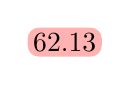
\begin{tikzpicture}[baseline=(X.base)]
\node[fill=red!30, inner sep=2pt, rounded corners] (X) {62.13};\end{tikzpicture} \\ 
\textbf{GPT-4o mini}   & 63.72 / 60.95 & 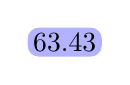
\begin{tikzpicture}[baseline=(X.base)]
\node[fill=blue!30, inner sep=2pt, rounded corners] (X) {63.43};\end{tikzpicture} / 60.15 & 53.85 / 52.46 & 50.01 / 47.75 & \textcolor{blue}{\textbf{66.91}} / \textcolor{red}{\textbf{61.08}} & 60.13 / 57.28 \\ 
\textbf{LLaMA3.3-70B}   & 68.13 / 63.96 & 62.12 / 60.32 & 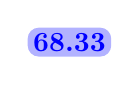
\begin{tikzpicture}[baseline=(X.base)]
\node[fill=blue!30, inner sep=2pt, rounded corners] (X) {\textcolor{blue}{\textbf{68.33}}};\end{tikzpicture} / 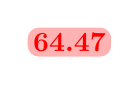
\begin{tikzpicture}[baseline=(X.base)]
\node[fill=red!30, inner sep=2pt, rounded corners] (X) {\textcolor{red}{\textbf{64.47}}};\end{tikzpicture} & 53.13 / 51.78 & 58.16 / 59.22 & 52.41 / 48.82 \\ 
\textbf{LLaMA3.3-8B}    & 58.97 / 61.11 & 56.19 / 55.98 & \textcolor{blue}{\textbf{63.24}} / \textcolor{red}{\textbf{63.72}} & 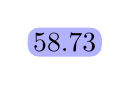
\begin{tikzpicture}[baseline=(X.base)]
\node[fill=blue!30, inner sep=2pt, rounded corners] (X) {58.73};\end{tikzpicture} / 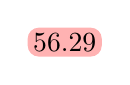
\begin{tikzpicture}[baseline=(X.base)]
\node[fill=red!30, inner sep=2pt, rounded corners] (X) {56.29};\end{tikzpicture} & 59.83 / 59.17 & 49.66 / 48.97 \\ 
\textbf{Qwen2-72B}      & 62.70 / 61.09 & 62.91 / 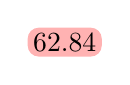
\begin{tikzpicture}[baseline=(X.base)]
\node[fill=red!30, inner sep=2pt, rounded corners] (X) {62.84};\end{tikzpicture} & 58.71 / 56.99 & 49.12 / 47.26 & 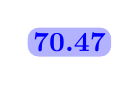
\begin{tikzpicture}[baseline=(X.base)]
\node[fill=blue!30, inner sep=2pt, rounded corners] (X) {\textcolor{blue}{\textbf{70.47}}};\end{tikzpicture} / 
\begin{tikzpicture}[baseline=(X.base)]
\node[fill=red!30, inner sep=2pt, rounded corners] (X) {\textcolor{red}{\textbf{67.98}}};\end{tikzpicture} & 61.24 / 58.18 \\ 
\textbf{Qwen2-7B}       & 63.78 / 61.54 & 58.11 / 57.84 & 60.15 / 58.60 & 48.72 / 49.17 & \textcolor{blue}{\textbf{65.44}} / \textcolor{red}{\textbf{63.58}} & 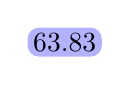
\begin{tikzpicture}[baseline=(X.base)]
\node[fill=blue!30, inner sep=2pt, rounded corners] (X) {63.83};\end{tikzpicture} / 61.91 \\ 
\bottomrule
\end{tabular}}
\caption{F1 scores of LLM-based detectors on human-annotated texts for \textbf{binary} classification. Each dataset contains 100 LGTs and 100 HGTs with human-annotated explanations. Each cell indicates classification/explanation F1, where the highest column-wise F1 of each LLM detector for binary classification and explanations across different generated texts are highlighted with \colorbox{blue!30}{blue} and \colorbox{red!30}{red}, respectively. In addition, the highest row-wise F1 among different LLM detectors for each LLM-generated text datasets are indicated with \textcolor{blue}{\textbf{blue}} and \textcolor{red}{\textbf{red}} in bold, respectively.}
% \vspace{-1em}
\label{tab:binary_annotate_performance}
\end{table*}

As shown in Table~\ref{tab:binary_mgt_hgt_performance}, analysis of the annotators' results revealed that models are generally more accurate in attributing HGTs compared to LGTs. For example, while GPT-4o demonstrates higher accuracy (78 out of 100) in classifying HGTs, the false explanations account for more than 47\%.

\begin{table*}[tb]
\centering
\footnotesize
\renewcommand{\arraystretch}{1.2} % 调整行间距
\resizebox{\textwidth}{!}{
% \begin{tabularx}{\textwidth}{@{}c *{3}{>{\centering\arraybackslash}X} *{3}{>{\centering\arraybackslash}X} *{3}{>{\centering\arraybackslash}X} *{3}{>{\centering\arraybackslash}X} @{}}
\begin{tabular}{lcccccccccccc}
\toprule
\multirow{2}{*}{Model} & \multicolumn{6}{c}{MGTs} & \multicolumn{6}{c}{HGTs} \\
\cmidrule(lr){2-4} \cmidrule(lr){5-7} \cmidrule(lr){8-10} \cmidrule(lr){11-13}
 & TC & TE & FE & FC & TE & FE & TC & TE & FE & FC & TE & FE \\
\midrule
GPT-4o & 64 & ${51}_{\textcolor{teal}{:79.7\%}}$ & ${13}_{\textcolor{teal}{:20.3\%}}$ & 36 & ${8}_{\textcolor{teal}{:22.2\%}}$ & ${28}_{\textcolor{teal}{:77.8\%}}$ & 78 & ${41}_{\textcolor{teal}{:52.6\%}}$ & ${37}_{\textcolor{teal}{:47.4\%}}$ & 22 & ${2}_{\textcolor{teal}{:9.1\%}}$ & ${20}_{\textcolor{teal}{:90.9\%}}$ \\
LLaMA3.3-70B & 56 & ${35}_{\textcolor{teal}{:62.5\%}}$ & ${21}_{\textcolor{teal}{:37.5\%}}$ & 44 & ${10}_{\textcolor{teal}{:22.7\%}}$ & ${34}_{\textcolor{teal}{:77.3\%}}$ & 60 & ${37}_{\textcolor{teal}{:61.7\%}}$ & ${23}_{\textcolor{teal}{:38.3\%}}$ & 40 & ${7}_{\textcolor{teal}{:17.5\%}}$ & ${33}_{\textcolor{teal}{:82.5\%}}$ \\
Qwen2-72B & 60 & ${36}_{\textcolor{teal}{:60.0\%}}$ & ${24}_{\textcolor{teal}{:40.0\%}}$ & 40 & ${7}_{\textcolor{teal}{:17.5\%}}$ & ${33}_{\textcolor{teal}{:82.5\%}}$ & 69 & ${50}_{\textcolor{teal}{:72.5\%}}$ & ${19}_{\textcolor{teal}{:27.5\%}}$ & 31 & ${7}_{\textcolor{teal}{:22.6\%}}$ & ${24}_{\textcolor{teal}{:77.4\%}}$ \\
\bottomrule
\end{tabular}}
\caption{Performance of LLMs on LLM-generated and human-generated texts for ternary classification and explanation tasks. It includes results for classification and explanation tasks, where TC represents true classification, FC represents false classification, TE represents true explanation, and FE represents false explanation. Note: TC=TE+FE and FC=TE+FE.}
% \vspace{-1.5em}
\label{tab:binary_mgt_hgt_performance}
\end{table*}

\begin{table}[tb]
\centering
\small
\begin{tabular}{@{}p{\linewidth}@{}} % 使用p{width}指定每列宽度
\toprule
\textbf{Prompt}: Please classify the following text into one of three categories based on its source: LLM-generated, human-generated, or undecided. The ``Undecided'' category refers to texts that exhibit characteristics of both LLM-generated and human-generated content, making it impossible and inappropriate to distinguish between the two. Provide a clear classification and a detailed explanation for your decision. Structure your answer in JSON format as follows: \{``classification'': , ``explanation'': \}.\\
\bottomrule
\end{tabular}
\caption{A prompt designed for LLMs to determine the origin of a text and provide an explanation under a ternary setting.}
% \vspace{-1.5em}
\label{tab:prompt_ternary_classification}
\end{table} 
\section{LLM-based Ternary Classification on LGTs and HGTs}

\subsection{Experimental Setup}

Using the same benchmark in Section~\ref{sec:binary_classification}, we prompted the LLMs for ternary classification and the prompt template is demonstrated in Table~\ref{tab:prompt_ternary_classification}. The ground truth for the ternary classification was determined based on annotators' votes, where the three annotators were aware of the text's origin (LLMs or human) and were asked to distinguish between the ground truth and the ``Undecided'' category. This allowed for the evaluation of both the LLM's classification results and the explanations provided by the LLMs. The Fleiss' kappa~\cite{Fleiss1971kappa} for the ternary classification annotations among the three annotators was calculated as 0.7629, which indicates substantial agreement.

\subsection{Ternary Classification Results}

Table~\ref{tab:ternary_performance} presents the F1 scores of LLMs in the ternary classification setting. Comparing it with Table~\ref{tab:binary_annotate_performance}, we observe that introducing the ``Undecided'' category leads to overall performance improvements across both classification and explanation tasks. Specifically, GPT-4o exhibits the most notable gains, improving from 73.48/67.04 to 79.73/72.04, indicating that a finer-grained classification allows stronger models to better capture nuanced differences between LGTs and HGTs.

\begin{table*}[tb]
\centering
\small
% \setlength{\tabcolsep}{3pt}
% \begin{tabularx}{\textwidth}{@{}c *{6}{>{\centering\arraybackslash}X} @{}}
\resizebox{\textwidth}{!}{
\begin{tabular}{lcccccc}
\toprule
\multirow{2}{*}{\diagbox{Datasets}{Models}} & \multicolumn{6}{c}{LLM Detectors}\\
& GPT-4o & GPT-4o mini & LLaMA3.3-70B & LLaMA3.3-8B & Qwen2-72B & Qwen2-7B \\
\midrule
\textbf{GPT-4o} & 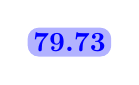
\begin{tikzpicture}[baseline=(X.base)]
\node[fill=blue!30, inner sep=2pt, rounded corners] (X) {\textcolor{blue}{\textbf{79.73}}};\end{tikzpicture}/\textcolor{red}{\textbf{72.04}} & 64.62/61.87 & 62.19/59.04 & 58.06/57.78 & 71.62/68.86 & 63.81/62.72 \\
\textbf{GPT-4o mini} & \textcolor{blue}{\textbf{70.11}}/\textcolor{red}{\textbf{68.75}} & 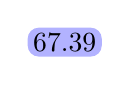
\begin{tikzpicture}[baseline=(X.base)]
\node[fill=blue!30, inner sep=2pt, rounded corners] (X) {67.39};\end{tikzpicture}/  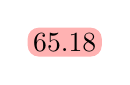
\begin{tikzpicture}[baseline=(X.base)]
\node[fill=red!30, inner sep=2pt, rounded corners] (X) {65.18};\end{tikzpicture} & 58.88/52.95 & 54.43/51.16 & 69.65/65.95 & 65.15/62.60 \\
\textbf{LLaMA3.3-70B} & \textcolor{blue}{\textbf{74.41}}/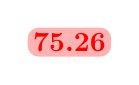
\begin{tikzpicture}[baseline=(X.base)]
\node[fill=red!30, inner sep=2pt, rounded corners] (X) {\textcolor{red}{\textbf{75.26}}};\end{tikzpicture} & 65.16/64.75 & 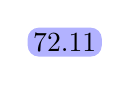
\begin{tikzpicture}[baseline=(X.base)]
\node[fill=blue!30, inner sep=2pt, rounded corners] (X) {72.11};\end{tikzpicture}/ 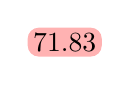
\begin{tikzpicture}[baseline=(X.base)]
\node[fill=red!30, inner sep=2pt, rounded corners] (X) {71.83};\end{tikzpicture} & 57.05/57.34 & 64.94/62.44 & 56.46/55.32 \\
\textbf{LLaMA3.3-8B} & \textcolor{blue}{\textbf{71.99}}/\textcolor{red}{\textbf{70.80}} & 60.18/61.10 & 64.82/63.93 & 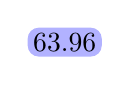
\begin{tikzpicture}[baseline=(X.base)]
\node[fill=blue!30, inner sep=2pt, rounded corners] (X) {63.96};\end{tikzpicture}/ 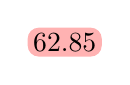
\begin{tikzpicture}[baseline=(X.base)]
\node[fill=red!30, inner sep=2pt, rounded corners] (X) {62.85};\end{tikzpicture} & 63.12/60.52 & 54.08/53.01 \\
\textbf{Qwen2-72B} & 67.28/66.74 & 65.12/64.73 & 61.81/61.74 & 53.24/52.87 & 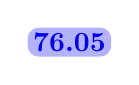
\begin{tikzpicture}[baseline=(X.base)]
\node[fill=blue!30, inner sep=2pt, rounded corners] (X) {\textcolor{blue}{\textbf{76.05}}};\end{tikzpicture}/ 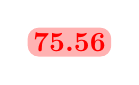
\begin{tikzpicture}[baseline=(X.base)]
\node[fill=red!30, inner sep=2pt, rounded corners] (X) {\textcolor{red}{\textbf{75.56}}};\end{tikzpicture} & 65.26/64.72 \\
\textbf{Qwen2-7B} & 68.91/67.42 & 60.15/59.31 & 62.06/61.57 & 52.41/52.30 & \textcolor{blue}{\textbf{70.30}}/\textcolor{red}{\textbf{68.44}} & 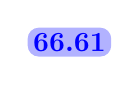
\begin{tikzpicture}[baseline=(X.base)]
\node[fill=blue!30, inner sep=2pt, rounded corners] (X) {\textcolor{blue}{\textbf{66.61}}};\end{tikzpicture}/ 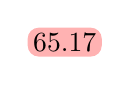
\begin{tikzpicture}[baseline=(X.base)]
\node[fill=red!30, inner sep=2pt, rounded corners] (X) {65.17};\end{tikzpicture} \\
\bottomrule
\end{tabular}}
\caption{F1 scores of LLM-based detectors on the \textbf{ternary} classification of LGTs and HGTs. The highest column-wise and row-wise F1 scores are highlighted and marked following the same scheme as in Table \ref{tab:binary_annotate_performance}.}
% \vspace{-1.5em}
\label{tab:ternary_performance}
\end{table*}

Moreover, Figure~\ref{fig:ternary_confusion_matrices} reveals how different models distribute predictions across the three categories. GPT-4o demonstrates a more balanced distribution, with relatively lower misclassification rates for both HGTs and LGTs. In contrast, LLaMA3-70B shows a stronger tendency to label texts as ``human-generated'', leading to a higher false positive rate. Meanwhile, Qwen2-72B exhibits a more cautious classification approach, assigning a larger proportion of texts to the ``Undecided'' category, particularly for LGTs.

\pgfplotsset{
    CM common axis styles/.style={
        width=1.8in,
        height=1.8in,
        xmajorgrids=false,
        ymajorgrids=false,
        xmin=1, xmax=3,
        ymin=1, ymax=3,
        xtick={1,2,3},
        ytick={1,2,3},
        xticklabels={LLMs, Undecided, Human},
        yticklabels={LLMs, Undecided, Human},
        x tick label style={font=\scriptsize},
        y tick label style={font=\scriptsize},
        tickwidth=0pt,
        tick align=outside,
        enlargelimits={abs=0.5},
        colormap={whiteblue}{rgb255(0cm)=(255,255,255) rgb255(1cm)=(128,128,255)}
        },
    CM common plot styles/.style={
        matrix plot,
        mesh/cols=3,
        mesh/rows=3,
        point meta=explicit,
        nodes near coords,
        nodes near coords align={center},
        visualization depends on={value \thisrow{q} \as \rawvalue},
        nodes near coords style={font=\tiny, color=black}
        }
}
\begin{figure*}[tb]
\begin{subfigure}{0.3\textwidth} % 修改子图的宽度为三分之一
    \centering
    \begin{tikzpicture}
    \begin{axis}[
    CM common axis styles
    ]
    \addplot [
    CM common plot styles
    ] table [meta=p] {
    x y p
    1 1 76.5
    2 1 10.4
    3 1 4.2
    1 2 12.3
    2 2 66.7
    3 2 36.6
    1 3 11.1
    2 3 22.9
    3 3 59.2
    };
    \end{axis}
    \end{tikzpicture}
    \caption{GPT-4o}
\end{subfigure}%
\begin{subfigure}{0.3\textwidth} % 修改子图的宽度为三分之一
    \centering
    \begin{tikzpicture}
    \begin{axis}[
    CM common axis styles
    ]
    \addplot [
    CM common plot styles
    ] table [meta=p] {
    x y p
    1 1 46.9
    2 1 18.8
    3 1 11.3
    1 2 18.5
    2 2 62.5
    3 2 16.9
    1 3 34.6
    2 3 18.8
    3 3 71.8
    };
    \end{axis}
    \end{tikzpicture}
    \caption{LLaMA3.3-70B}
\end{subfigure}%
\begin{subfigure}{0.3\textwidth} % 修改子图的宽度为三分之一
    \centering
    \begin{tikzpicture}
    \begin{axis}[
    CM common axis styles,
    colorbar, % 仅保留此处的 colorbar
    colorbar style={
        width=2mm, % 设置 colorbar 的宽度
        ytick={0, 20, 40, 60, 80, 100},
        yticklabel style={font=\scriptsize},
        title=\%,
        title style={
            yshift=-2mm  % 向下移动标题的位置
        }
    },
    point meta min=0,
    point meta max=100
    ]
    \addplot [
    CM common plot styles
    ] table [meta=p] {
    x y p
    1 1 75.3
    2 1 35.4
    3 1 16.9
    1 2 3.7
    2 2 43.8
    3 2 18.3
    1 3 21.0
    2 3 20.8
    3 3 64.8
    };
    \end{axis}
    \end{tikzpicture}
    \caption{Qwen2-72B}
\end{subfigure}
\caption{Confusion matrices showing the performance of LLM-based detectors (GPT-4, LLaMA3.3-70B, Qwen2-72B) in the ternary classification task, where the bottom row represents human-annotated ground truth labels (LGTs, Undecided, and HGTs), and the left column represents classification results predicted by LLM-based detectors.}
%\vspace{-1.5em}
\label{fig:ternary_confusion_matrices}
\end{figure*}

A closer comparison between the binary and ternary classification results in Tables~\ref{tab:binary_annotate_performance} and \ref{tab:ternary_performance} suggests that the added ``Undecided'' category benefits models differently. While large-scale models like GPT-4o and LLaMA3-70B leverage this additional flexibility to improve both classification and explanation F1 scores, smaller models such as Qwen2-7B show more mixed results, with only marginal improvements. This suggests that high-capacity models may be better equipped to handle ambiguous cases, while smaller models can struggle with the added complexity.

Overall, these findings indicate that ternary classification not only refines detection performance but also enhances the LLMs' ability to generate more meaningful explanations. The improvements are particularly evident in large-scale LLMs, which benefit from a more nuanced decision space.

\section{Explainability of LLM-based Detectors}

\subsection{Incorrect Explanation Attribution}

Although LLMs can distinguish LGTs and HGTs, especially in self-detection settings, there are explanations that are incorrect via human evaluation. Normally, incorrect explanations in correctly classified cases fall into three types: inaccurate features (misidentifying key attributes), hallucinations (citing nonexistent or contradictory features), and flawed reasoning (faulty logic despite a correct outcome). For misclassified texts, errors typically involve inaccurate features or hallucinations, which highlights the need to prioritize explanation accuracy alongside detection performance to enhance trust in LLM-based detectors.

\subsubsection{Inaccurate Features}

Incorrect explanation attribution is often caused by relying on ambiguous, superficial, or misinterpreted features, as shown in the examples in Tables~\ref{tab:main_misattributions_examples} and \ref{tab:misattributions_examples} of Appendix~\ref{appendix:misattributions_examples}.

In Example 1 ``Ambiguous Features'', the model misclassifies a text on quantum entanglement as LGTs due to the use of technical jargon. However, advanced topics can also be written by human experts, not just LLMs. This text was actually human-generated. Similarly, Example 2 ``Surface Features'' shows how the model links grammatical errors to machine authorship. Such mistakes are common among both native and non-native writers and should not be sole indicators of LGTs. In fact, HGTs are more likely to contain grammatical errors.

Example 3 illustrates a misjudgment where emotional complexity is falsely attributed exclusively to human writing. The model assumes nuanced emotional contrasts inherently reflect human authorship, overlooking modern LLMs' capability to simulate such depth. This case underscores the unreliability of using emotional sophistication alone as a criterion to differentiate between HGTs and LGTs.

\begin{table*}[tb]
\centering
\small
\begin{tabular}{@{}p{\linewidth}@{}}
\toprule
\textbf{Example 1: Ambiguous Features}

\textbf{Original Text}: ``Quantum entanglement enables faster-than-light communication, allowing for instantaneous data transfer across vast distances. This phenomenon has vast implications for future communication technologies, making it a subject of growing interest in both academic and technological circles.''

\textbf{LLM Judgment}: LLM-generated

\textbf{LLM Explanation}: ``The text discusses highly technical content, filled with specialized scientific terms, which is characteristic of machine-generated text. Such advanced topics are often produced by AI systems rather than human experts.''\\

\midrule

\textbf{Example 4: Incorrectly Perceived Repetition}

\textbf{Original Text}: ``The discovery of gravitational waves was a turning point in the history of physics. This breakthrough confirmed Einstein’s theory of relativity, providing compelling evidence for the existence of gravitational waves, which opened new doors in astrophysics research.''

\textbf{LLM Judgment}: LLM-generated

\textbf{LLM Explanation}: ``The text exhibits repetitive sentence structures, a hallmark of AI-generated content. The repeated mention of 'gravitational waves' and 'breakthrough' indicates a pattern commonly seen in machine-generated texts.''\\

\midrule

\textbf{Example 6: Misinterpretation of Formal Tone}

\textbf{Original Text}: ``One must consider the economic ramifications of such policies, as they extend beyond immediate financial concerns into broader societal impacts. The implications of these policies are far-reaching, touching on employment, income inequality, and long-term societal well-being.''

\textbf{LLM Judgment}: LLM-generated

\textbf{LLM Explanation}: ``The formal tone and structured language initially suggest human authorship, as such features are often attributed to human experts. However, LLMs can replicate this style with high fidelity, leading to the final classification as LLM-generated.''\\

\bottomrule
\end{tabular}
\caption{Analysis of LLM vs. Human Writing Attribution Based on Various Features. The table categorizes examples where LLM-generated and human-written texts were incorrectly attributed or analyzed, providing explanations and analyses of these misattributions.}
\vspace{-1.5em}
\label{tab:main_misattributions_examples}
\end{table*}

\subsubsection{Hallucinations}

Hallucinations occur when the model incorrectly attributes features to the text that either do not exist or are contrary to the actual content. In Example 4: Incorrectly Perceived Repetition, the model misinterprets the repetition of ideas about gravitational waves as a sign of LLM authorship. The text does not exhibit excessive repetition, and the claim of a repetitive structure is a false attribution, likely due to biases in the model’s training data.

In Example 5: Fictitious Absence of Domain Knowledge, the model mistakenly claims that a text about RNA interference lacks technical depth, suggesting it is more likely to be human-written. In reality, the text contains domain-specific biological content, and the model fails to recognize the technical knowledge present.

\subsubsection{Incorrect Reasoning}

Incorrect reasoning occurs when relevant features are correctly identified but are misinterpreted, leading to incorrect conclusions. Example 6 highlights a classification error rooted in inconsistent reasoning. The model correctly identifies formal stylistic features but misapplies their significance. Enforcing a binary classification may lead to inconsistent reasoning in the model’s inference process, as it forces an erroneous LLM label despite the ambiguity that could be better captured in a ternary framework.

\subsection{Human Evaluation to Incorrect Explanations}

The reasons for incorrect explanations from human annotators are categorized into two scenarios: correct predictions with incorrect explanations and incorrect predictions with incorrect explanations. The results are summarized in Tables~\ref{tab:correct_but_wrong_explanation} and \ref{tab:incorrect_and_wrong_explanation}.

For cases where the model made correct predictions but provided incorrect explanations, Table~\ref{tab:correct_but_wrong_explanation} shows that the most prevalent reasons were inaccurate features and hallucinations. Inaccurate features, such as attributing the decision to vague or irrelevant characteristics, accounted for a significant portion of errors across all LLMs. Hallucinations were also frequent, particularly for models like Qwen2-7B and GPT-4o. Faulty reasoning, though less common, contributed to the proportion of incorrect explanations, highlighting inconsistencies in reasoning despite identifying correct features.

For cases involving both incorrect predictions and incorrect explanations, Table~\ref{tab:incorrect_and_wrong_explanation} indicates a similar distribution of error types, but with a higher prevalence of hallucinations. Annotators noted that models hallucinated key features, attributing the decision to features not present in the text, which compounded the issue of misclassification. 

Overall, the analysis reveals that hallucinations and reliance on inaccurate features are dominant sources of error in explanations, regardless of prediction accuracy. Addressing these issues requires further refinement of the interpretability mechanisms in LLMs, with a focus on grounding explanations in verifiable and relevant textual evidence.

\begin{table*}[tb]
\centering
\small
% \setlength{\tabcolsep}{3pt}
% \begin{tabularx}{\textwidth}{@{}c *{6}{>{\centering\arraybackslash}X} @{}}
\resizebox{\textwidth}{!}{
\begin{tabular}{lcccccc}
\toprule
Models & Ambiguous Features (\%) & Surface Features (\%) & Logic\&Emotion (\%) & Vocabulary (\%) & Hallucinations (\%) & Incorrect Reasoning (\%)\\
\midrule
GPT-4o & 32.7 & 12.4 & 43.2 & 7.2 & 2.2 & 2.3\\
LLaMA3.3-70B & 40.1 & 25.7 & 18.9 & 4.1 & 6.1 & 5.1\\
Qwen2-72B & 32.1 & 23.7 & 25.4 & 8.9 & 6.3 & 3.6\\
\bottomrule
\end{tabular}}
\caption{Attribution differences among LLMs when the judgment is correct but the explanation is incorrect.}
%\vspace{-0.5em}
\label{tab:correct_but_wrong_explanation}
\end{table*}

\begin{table*}[tb]
\centering
\small
% \begin{tabularx}{\textwidth}{@{}c *{5}{>{\centering\arraybackslash}X} @{}}
\resizebox{\textwidth}{!}{
\begin{tabular}{lccccc}
\toprule
Models & Ambiguous Features (\%) & Surface Features (\%) & Logic\&Emotion (\%) & Vocabulary (\%) & Hallucinations (\%)\\
\midrule
GPT-4o & 13.9 & 30.7 & 23.8 & 20.7 & 10.9\\
LLaMA3.3-70B & 26.8 & 10.1 & 40.1 & 4.1 & 18.9\\
Qwen2-72B & 33.7 & 20.1 & 9.9 & 26.4 & 9.9\\
\bottomrule
\end{tabular}}
\caption{Attribution differences among LLMs when both the judgment and the explanation are incorrect.}
\vspace{-1.5em}
\label{tab:incorrect_and_wrong_explanation}
\end{table*}

\section{Discussion}

\subsection{Can Fine-Tuning Enhance Cross-LLM Detection Performance?}

To explore whether fine-tuning improves cross-LLM detection, we fine-tuned Qwen2-7B on a training set consisting of 10,000 LLaMA3.3-8B-generated LGTs and 10,000 HGTs from M4GT-Bench dataset using Low-Rank Adaptation (LoRA) \cite{hu2021lora} for the binary classification task. Table~\ref{tab:fine_tune_qwen} demonstrates a performance decrease of Qwen2-7B's self-detection on Qwen2-7B’s dataset, while there was a marginal improvement on LLaMA3.3-8B’s dataset of Qwen2-7B's cross-detection. This indicates that simple fine-tuning might not significantly improve LLM's cross-detection performance, and even bring a damage to its self-detection. The observed changes can be attributed to two primary factors:

\begin{table}[tb]
\small
\centering 
% \begin{tabularx}{0.48\textwidth}{@{}c *{2}{>{\centering\arraybackslash}X} @{}}
\resizebox{\columnwidth}{!}{
\begin{tabular}{lcc}
\toprule 
\diagbox{Model}{Datasets} & Qwen2-7B & LLaMA3.3-8B\\
\midrule 
Qwen2-7B & -4.31\% / -6.50\% & +0.19\% / -3.20\%\\
\bottomrule 
\end{tabular}} 
\caption{Results of fine-tuning Qwen2-7B. The first and second F1 scores indicate the accuracy difference in classification and explanation accuracy compared to the original model, respectively.}
%\vspace{-1.5em}
\label{tab:fine_tune_qwen} 
\end{table}

\paragraph{Overfitting on the New Dataset:} The training set may not have sufficiently captured the distinct features of LLaMA3.3-8B, which leads to overfitting on the training data and a decrease in generalization. 
% This is reflected in the decrease in performance on Qwen2-7B’s dataset.

\paragraph{Catastrophic Forgetting of Original LLMs:} Fine-tuning may cause Qwen2-7B to lose some of its inherent language capabilities. By specializing in cross-detection, Qwen2-7B experiences ``catastrophic forgetting'', where previously learned knowledge is overwritten, which reduces overall language proficiency. This is evident in the decline of both detection and explanation accuracy after fine-tuning.

Furthermore, the decrease in explanation accuracy on both models after fine-tuning, alongside the reduced detection performance on Qwen2-7B's dataset, indicates that simple finetuning does not lead to substantial improvements. Instead, it may have negative effects to damage the model's reasoning ability. 
% This outcome highlights the limitations of current fine-tuning methods, which typically focus only on classification without considering explanations.

% Given that many current fine-tuning methods only optimize classification, the results indicate that integrating explanation accuracy into fine-tuning is a promising future direction. A combined approach of fine-tuning both detection and explanation could potentially lead to more balanced performance improvements, particularly for cross-LLM detection tasks.

\subsection{Enhancing LLM Detection through LLM Collaboration}

We further explore whether the performance of LLM-based detection can improve via LLM's collaboration. Table~\ref{tab:model_collaboration} shows that the performance of LLM-based detectors improves significantly when their judgments and explanations are complemented by another LLM counterpart. Specifically, the cross-detection of GPT-4o on Qwen-2 72B dataset has noticeable improvements in the classification and explanation F1 with the support of Qwen2-72B. We also find a similar trend, where Qwen2-72B benefits from GPT-4o's support on the cross-detection settings. These findings indicate that LLM's collaboration can further improve the classification and explanation performance on the LLM  counterpart's dataset, i.e., cross-detection.

% Model collaboration, especially between larger and smaller models, enhances not only detection capabilities but also the quality of explanations. These findings suggest that leveraging multiple models’ outputs can refine detection performance. For details, see Table~\ref{tab:model_collaboration}.

\begin{table}[ht] 
\small 
\centering 
\resizebox{\columnwidth}{!}{
 \begin{tabular}{lcc}
\toprule 
\diagbox{Models}{Datasets} & GPT-4o & Qwen2-72B\\
\midrule 
GPT-4o (+Qwen2-72B) & +1.43\% / -0.61\% & +3.79\% / +2.33\%\\
Qwen2-72B (+GPT-4o) & +2.01\% / +0.45\% & +0.39\% / -1.24\%\\
\bottomrule 
\end{tabular} 
}
\caption{F1 score differences based on LLM collaboration with judgments and explanations integration. The supplemental LLMs in () will generate the judgments and explanations first to further support the detection and explanations of main LLMs.} 
%\vspace{-1.5em}
\label{tab:model_collaboration} 
\end{table}



\section{Conclusion}

We evaluated how well LLM-based detectors differentiate human- from LLM-generated text, focusing on detection accuracy and explanation clarity. Overall, self-detection outperformed cross-detection, and detectors within the same model series tended to behave better. However, explanation quality lagged, often relying on flawed features, hallucinations, and poor reasoning. Distinct error patterns emerged: GPT-4o showed high accuracy yet frequent hallucinations, while Qwen2-7B struck a better accuracy-explanation balance but often used vague features. These findings underscore the need for interpretable, trustworthy detectors, particularly in high-stakes contexts like academic integrity and content moderation.



\section*{Limitations}

This study is subject to several limitations. First, due to the limited number of API calls available for closed-source LLMs, the datasets used for generating and detecting LLM-generated texts were constructed at a scale of 1,000 samples. As a result, the types and variety of texts involved in the analysis may not be fully comprehensive, potentially introducing bias. Additionally, because the generation of explanations requires manual annotation, which is time-consuming, only a random sample of 100 texts per dataset could be selected for evaluation. This sample size may lead to biases in the evaluation of LLM-generated explanations. Finally, given the rapid advancements in LLM technology, the detection and explanation capabilities of models are continually evolving. Therefore, it is crucial to periodically update our research focus and the models under study to ensure the results remain relevant and accurate.

\section*{Ethic Statements}

All experiments were conducted using publicly available LLMs and datasets. For the datasets we constructed for the work, no any personal or private information is included. All the three human annotators are co-authors, so an research ethics review was not considered necessary. More details on how we used the human annotators can be found in Appendix~\ref{appendix:annotation_guidelines}.

% Bibliography entries for the entire Anthology, followed by custom entries
%\bibliography{anthology,custom}
% Custom bibliography entries only
\bibliography{main}

\appendix

\section{Misattributions Examples}
\label{appendix:misattributions_examples}

To better illustrate the types of errors and their attributions, Table~\ref{tab:misattributions_examples} provides examples of common mistakes made by the models in classifying text origins.

\begin{table*}[h]
\centering
\small
\begin{tabular}{@{}p{\linewidth}@{}}
\toprule
% \textbf{Example 1: Ambiguous Features}

% \textbf{Original Text}: ``Quantum entanglement enables faster-than-light communication, allowing for instantaneous data transfer across vast distances. This phenomenon has vast implications for future communication technologies, making it a subject of growing interest in both academic and technological circles.''

% \textbf{LLM Judgment}: LLM-generated

% \textbf{LLM Explanation}: ``The text discusses highly technical content, filled with specialized scientific terms, which is characteristic of machine-generated text. Such advanced topics are often produced by AI systems rather than human experts.''\\

% \midrule

\textbf{Example 2: Surface Features}

\textbf{Original Text}: ``The book were interesting. It show a deep exploration of human emotions and relationships. The author’s use of metaphors and descriptive language provided rich insights into the human psyche, but the writing style seemed awkward and unpolished in places.''

\textbf{LLM Judgment}: LLM-generated

\textbf{LLM Explanation}: ``The grammatical errors such as 'were' instead of 'was' and 'show' instead of 'shows' suggest that the text is AI-generated. Machines typically generate text with such mistakes.''\\

\midrule

\textbf{Example 3: Misattributed Logical or Emotional Elements}

\textbf{Original Text}: ``His words carried a strange contradiction—he spoke of hope but with an undeniable sadness. It was as though the optimism in his tone clashed with his deeply melancholic gaze, creating a complex emotional paradox.''

\textbf{LLM Judgment}: Human-written

\textbf{LLM Explanation}: ``The nuanced contradiction of hope and sadness reflects deeply human emotional complexity, which LLMs typically struggle to replicate authentically. Such layered emotional depth is often unique to human expression.''\\

\midrule

% \textbf{Example 4: Incorrectly Perceived Repetition}

% \textbf{Original Text}: ``The discovery of gravitational waves was a turning point in the history of physics. This breakthrough confirmed Einstein’s theory of relativity, providing compelling evidence for the existence of gravitational waves, which opened new doors in astrophysics research.''

% \textbf{LLM Judgment}: LLM-generated

% \textbf{LLM Explanation}: ``The text exhibits repetitive sentence structures, a hallmark of AI-generated content. The repeated mention of 'gravitational waves' and 'breakthrough' indicates a pattern commonly seen in machine-generated texts.''\\

% \midrule

\textbf{Example 5: Fictitious Absence of Domain Knowledge}

\textbf{Original Text}: ``RNA interference plays a crucial role in gene regulation, allowing for targeted suppression of specific genetic sequences. This mechanism is being studied for its potential therapeutic applications in cancer treatment and genetic disorders.''

\textbf{LLM Judgment}: Human-written

\textbf{LLM Explanation}: ``The text lacks the level of technical depth and domain-specific knowledge typically found in professional scientific writing, suggesting that it is more likely to be written by a human author who is not an expert in the field.''\\

% \midrule

% \textbf{Example 6: Misinterpretation of Formal Tone}

% \textbf{Original Text}: ``One must consider the economic ramifications of such policies, as they extend beyond immediate financial concerns into broader societal impacts. The implications of these policies are far-reaching, touching on employment, income inequality, and long-term societal well-being.''

% \textbf{LLM Judgment}: LLM-generated

% \textbf{LLM Explanation}: ``The formal tone and structured language initially suggest human authorship, as such features are often attributed to human experts. However, LLMs can replicate this style with high fidelity, leading to the final classification as LLM-generated.''\\

\bottomrule
\end{tabular}
\caption{Analysis of LLM vs. Human Writing Attribution Based on Various Features. The table categorizes examples where LLM-generated and human-written texts were incorrectly attributed or analyzed, providing explanations and analyses of these misattributions.}
\label{tab:misattributions_examples}
\end{table*}

\section{Detailed Results after Fine-Tuning}
\label{appendix:sft_results}

We fine-tuned Qwen2-7B on a training set consisting of 10,000 LLaMA3.3-8B-generated LGTs and 10,000 HGTs from the M4GT-Bench dataset using Low-Rank Adaptation (LoRA)\cite{hu2021lora} for the binary classification task. After fine-tuning, the model's performance was evaluated on the overall dataset, with results indicating a decline in both detection and explanation accuracy, as shown in Table~\ref{tab:fine_tune_detailed}. Specifically, the fine-tuned model exhibited a decrease in both detection effectiveness and explanation clarity across all data.

\begin{table*}[tb]
\centering
\small
\resizebox{\textwidth}{!}{
\begin{tabular}{lcccccc}
\toprule
\diagbox{Models}{Datasets} & GPT-4o & GPT-4o mini & LLaMA3.3-70B & LLaMA3.3-8B & Qwen2-72B & Qwen2-7B\\
\midrule
\textbf{Qwen2-7B} & -1.29\% / -2.17\% & +0.04\% / -2.23\% &  +0.16\% / -1.35\% & +0.19\% / -3.20\% & -5.83\% / -6.02\% & -4.31\% / -6.50\%\\
\bottomrule
\end{tabular}}
\caption{Results of fine-tuning Qwen2-7B. The first and second F1 scores indicate the changes in classification and explanation accuracy, respectively, compared to the original model across all datasets.}
%\vspace{-1.5em}
\label{tab:fine_tune_detailed}
\end{table*}

\section{Annotation Guidelines}
\label{appendix:annotation_guidelines}

This appendix provides detailed instructions for the manual annotation tasks conducted in our study. The annotation process consists of two tasks: (1) a binary classification task to evaluate the accuracy of LLM-generated explanations, and (2) a ternary classification task where annotators evaluate both the correctness of the LLM's ternary classification judgments and the accuracy of its explanations based on known text sources.

\begin{table*}[h]
\centering
\small
\begin{tabular}{@{}p{\linewidth}@{}}
\toprule
\textbf{Task 1: Explanation Accuracy Evaluation}\\
Annotators will assess whether the explanation provided by the model correctly justifies its classification decision. Each explanation should be judged based on its logical consistency, relevance to the text, and whether it accurately reflects distinguishing features.\\

\textbf{Columns:}
\begin{itemize}
    \item \textbf{Text}: The text sample to be classified.
    \item \textbf{Detection Result}: The model’s classification of the text as ``LLM-generated'' or ``Human-generated.''
    \item \textbf{Model’s Explanation}: The explanation provided by the model for its classification decision.
    \item \textbf{Annotation}: Label the explanation as ``Accurate'' or ``Inaccurate'' based on its reasoning quality.
\end{itemize}\\

\textbf{Example:}\\
\textbf{Text}: ``In recent years, artificial intelligence has demonstrated remarkable progress, influencing numerous industries, including healthcare, finance, and creative writing. Many experts believe that this rapid advancement will continue to reshape the workforce and redefine human-machine collaboration.''\\
\textbf{Detection Result}: LLM-generated\\
\textbf{Model’s Explanation}: ``The highly structured argumentation and precise yet impersonal tone indicate that this text was likely machine-generated rather than composed by a human writer.''\\
\textbf{Annotation}: Inaccurate (While structured argumentation is common in LLM-generated text, human authors can also produce similarly structured and objective writing.)\\
\midrule

\textbf{Task 2: Ternary Classification with Explanation Evaluation}\\
Annotators will classify each text as ``LLM-generated,'' ``Human-generated,'' or ``Undecided,'' and evaluate whether the model’s explanation correctly justifies the classification. The ``Undecided'' label applies when the text lacks sufficient distinguishing features.\\

\textbf{Columns:}
\begin{itemize}
    \item \textbf{Text}: The text sample to be classified.
    \item \textbf{Detection Result}: LLM’ judgment of whether the text is ``LLM-generated,'' ``Human-generated,'' or ``Undecided.''
    \item \textbf{Model’s Explanation}: The explanation provided by the model.
    \item \textbf{Classification Annotation}: Label whether the model’s classification is ``Correct'' or ``Incorrect.''
    \item \textbf{Explanation Annotation}: Label the explanation as ``Accurate'' or ``Inaccurate'' based on its reasoning quality.
\end{itemize}\\

\textbf{Example:}\\
\textbf{Text}: ``Quantum mechanics, a field of physics that describes the behavior of particles at the atomic and subatomic levels, has led to groundbreaking discoveries such as quantum entanglement and superposition. These principles have paved the way for advancements in quantum computing and cryptography, revolutionizing modern technology.''\\
\textbf{Detection Result}: Undecided\\
\textbf{Model’s Explanation}: ``The text presents factual scientific content in a neutral tone, making it difficult to distinguish between human and machine authorship.''\\
\textbf{Classification Annotation}: Correct\\
\textbf{Explanation Annotation}: Accurate (The explanation correctly justifies why the text is indistinguishable.)\\
\bottomrule
\end{tabular}
\caption{Human Annotation Instructions}
\label{tab:annotation_instructions}
\end{table*}

\end{document}

